\documentclass[border=3pt,tikz]{standalone}
\usetikzlibrary{arrows}
\usetikzlibrary{positioning}
\usetikzlibrary{calc}
\usetikzlibrary{arrows}
\begin{document}
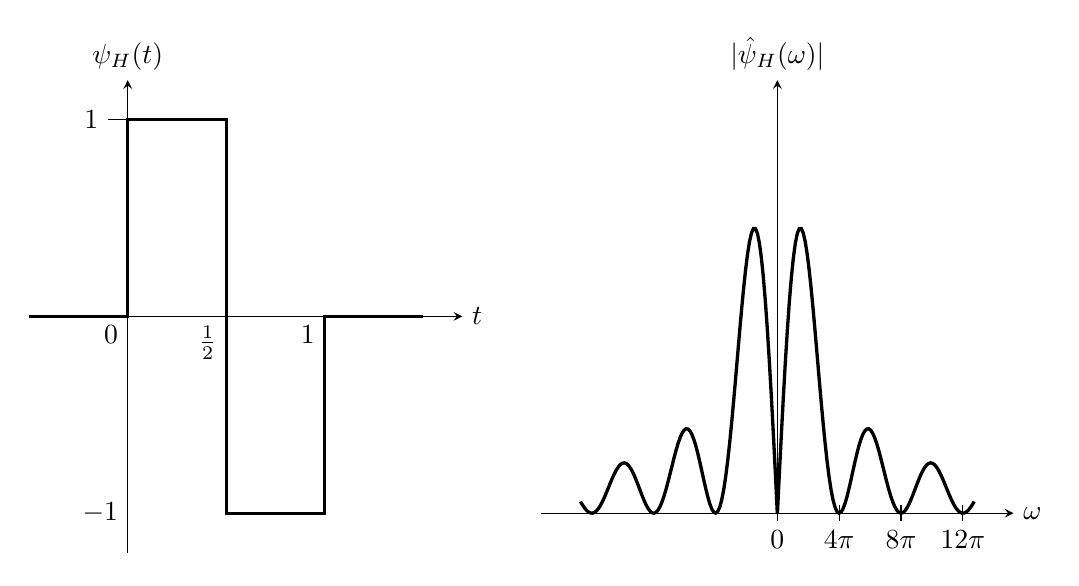
\begin{tikzpicture}[samples = 100, scale=2.5]

    \draw[-{stealth}] (-0.5, 0) -- (1.7,0) node[right] {$t$};
    \draw[-{stealth}] (0,-1.2) -- (0,1.2) node[above] {$\psi_H(t)$};
    
    \draw[very thick] (-0.5, 0) -- (0, 0) -- (0, 1) -- (0.5, 1) -- (0.5, -1) -- (1, -1)-- (1, 0) -- (1.5, 0);
    \node[] at (0, 0) [below left] {$0$};
    \node[] at (0.5, 0) [below left] {$\frac{1}{2}$};
    \node[] at (1, 0) [below left] {$1$};
    \draw[] (0.1, 1) -- (-0.1, 1) node[left] {$1$};
    \node[] at (0, -1) [left] {$-1$};
    
    \begin{scope}[xshift=3.3cm] 
    
    \draw[-{stealth}] (-1.2, -1) -- (1.2,-1) node[right] {$\omega$};
    \draw[-{stealth}] (0,-1.0) -- (0,1.2) node[above] {$|\hat{\psi}_H(\omega)|$};
    
    \draw[color=black, very thick, domain=0.01:40, samples=100, variable = \t]   plot ({\t/40}, {(2*(sin(\t*180/pi/4))*(sin(\t*180/pi/4)) / (\t/4)-1)});
    \draw[color=black, very thick, domain=-40:-0.01, samples=100, variable = \t]   plot ({\t/40}, {(-2*(sin(\t*180/pi/4))*(sin(\t*180/pi/4)) / (\t/4)-1)});
    \draw[] (0.0, -0.96) -- (0.0, -1.04 ) node[below] {$0$};
    \draw[] (0.314, -0.96) -- (0.314, -1.04 ) node[below] {$4\pi$};
    \draw[] (0.628, -0.96) -- (0.628, -1.04 ) node[below] {$8\pi$};
    \draw[] (0.942, -0.96) -- (0.942, -1.04 ) node[below] {$12\pi$};
    
    \end{scope}
    
    \end{tikzpicture}
\end{document}